Экспорт конфигурации виртуальной машины происходит в файл формата .ova (Open Virtual Appliance).

Это универсальный формат для хранения данных виртуальной машины, файлы .ova могут использоваться в разных программах виртуализации: VirtualBox, VMware Workstation, Microsoft Hyper-V. Виртуальная машина, экспортированная в файл .ova, затем может быть импортирована как в VirtualBox, так и в VMware Workstation, Microsoft Hyper-V.

В меню программы нужно зайти в «Файл» и выбрать пункт «Экспорт конфигураций». В открывшемся окне выбираем машину для экспорта, и нажимаем «Далее».

\begin{figure}[h]
		\centering
		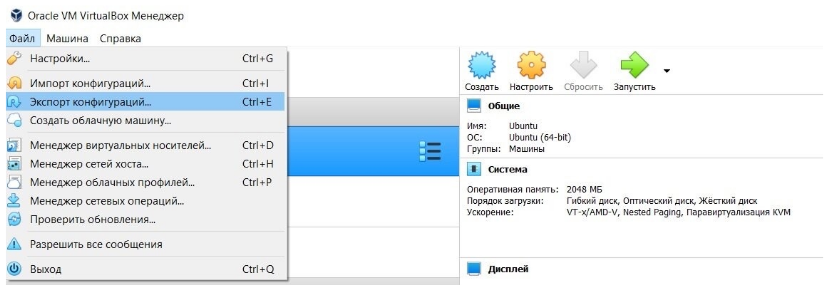
\includegraphics[width=1\linewidth]{VM/12.png}
\caption{«Экспорт конфигураций».}
\label{ris:image}

\end{figure}

Затем выбираем место размещения файла после экспорта. Также лучше выбрать пункт «Включать МАС-адреса всех сетевых адаптеров» и затем нажимаем «Далее». 

\begin{figure}[h]
		\centering
		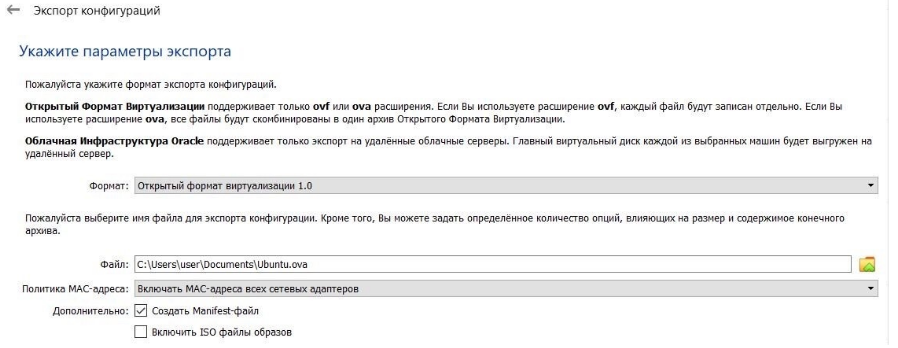
\includegraphics[width=1\linewidth]{VM/13.png}
\caption{МАС-адреса сетевых адаптеров.}
\label{ris:image}
\end{figure}

В следующем окне оставляем всё без изменений, и нажимаем кнопку “Экспорт”. Сам экспорт может занимать несколько минут, в зависимости от размера виртуальной машины. 

После экспорта в указанном месте создается файл, который уже необходимо будет импортировать.